\documentclass{beamer}
\setbeamertemplate{navigation symbols}{}
\mode<presentation> {
\usetheme{Berlin}
\usecolortheme{seahorse}
\setbeamertemplate{footline}[page number] 
}


\usepackage[style=ieee]{biblatex} % 
\usepackage{multicol}
\usepackage{graphicx} % Allows including images
\usepackage{booktabs} % Allows the use of \toprule, \midrule and \bottomrule in tables
\usepackage{tikz} % For flow diagrams etc.
\usepackage[T1]{fontenc} % use T1 fonts
\usepackage{amsmath} % nice math symbols
\usepackage{bm} % bold math
\usepackage{color} % change text color        
\usepackage{neuralnetwork}
\usepackage{tikz}
\usetikzlibrary{decorations.pathmorphing} % for snake lines
\usetikzlibrary{matrix} % for block alignment
\usetikzlibrary{arrows} % for arrow heads
\usetikzlibrary{calc} % for manimulation of coordinates
\usepackage{comment}
\includecomment{toexclude}
%\excludecomment{toexclude}


% TikZ styles for drawing
\tikzstyle{block} = [draw,rectangle,thick,minimum height=2em,minimum width=2em]
\tikzstyle{sum} = [draw,circle,inner sep=0mm,minimum size=2mm]
\tikzstyle{connector} = [->,thick]
\tikzstyle{line} = [thick]
\tikzstyle{branch} = [circle,inner sep=0pt,minimum size=1mm,fill=black,draw=black]
\tikzstyle{guide} = []
\tikzstyle{snakeline} = [connector, decorate, decoration={pre length=0.2cm,
                         post length=0.2cm, snake, amplitude=.4mm,
                         segment length=2mm},thick, magenta, ->]

%\bibliographystyle{ieee}
%Setup bibliography sources
\addbibresource{feiern.bib}


%----------------------------------------------------------------------------------------
%	TITLE PAGE
%----------------------------------------------------------------------------------------

%\title[RTNs]{Radio Transformer Networks} % The short title appears at the bottom of every slide, the full title is only on the title page
\title[OFDM_NN]{Mixing Old and New with Neural Networks in Communications} % The short title appears at the bottom of every slide, the full title is only on the title page

\author{Peter Hartig} % Your name
%\institute[FAU] % Your institution as it will appear on the bottom of every slide, may be shorthand to save space
%{
%FAU\\ % Your institution for the title page
%\medskip
%\textit{peter.hartig@fau.de} % Your email address
%}
\date{\today} % Date, can be changed to a custom date

\begin{document}

\begin{frame}
\titlepage % Print the title page as the first slide
\end{frame}

\section{Background} 



%------------------------------------------------

\subsection{Neural Networks} 

\begin{frame}
\frametitle{Overview} % Table of contents slide, comment this block out to remove it
\tableofcontents[currentsection,hideothersubsections,currentsubsection,
	subsubsectionstyle=hide
	] % Throughout your presentation, if you choose to use \section{} and \subsection{} commands, these will automatically be printed on this slide as an overview of your presentation
\end{frame}


\subsubsection{Building Blocks}
%NN ref https://github.com/battlesnake/neural
\begin{frame}[fragile]
\frametitle{Building Blocks: Single Neuron}
\begin{columns}
	\begin{column}{0.4\textwidth}
	    \begin{neuralnetwork}[height=4]
		\newcommand{\x}[2]{$x_#2$}
		\newcommand{\y}[2]{$\hat{y}_#2$}
		\inputlayer[count=3, bias=True, title=Input\\layer, text=\x]
		\outputlayer[count=1, title=Output\\layer, text=\y] \linklayers
	    \end{neuralnetwork}
	\end{column}

	\begin{column}{0.5\textwidth}
		\begin{figure}
			\begin{equation*}
				Output = f(\sum_{n=1}^{3} w_i*i_i+ bias)
			\end{equation*}
		\end{figure}

		\begin{small}
			Activation function incorporates non-linearity so long as there is tractable
			 $\Delta f()$ with respect to $w_{i,j}$.  Without non-linear functions, a network of arbitrary
			 depth can be collapsed to a single layer .
			\cite{baldi1989neural}
		\end{small}
	\end{column}
\end{columns}
\end{frame}


\begin{frame}[fragile]
\frametitle{Activation Functions: Sigmoid}
\begin{figure}
		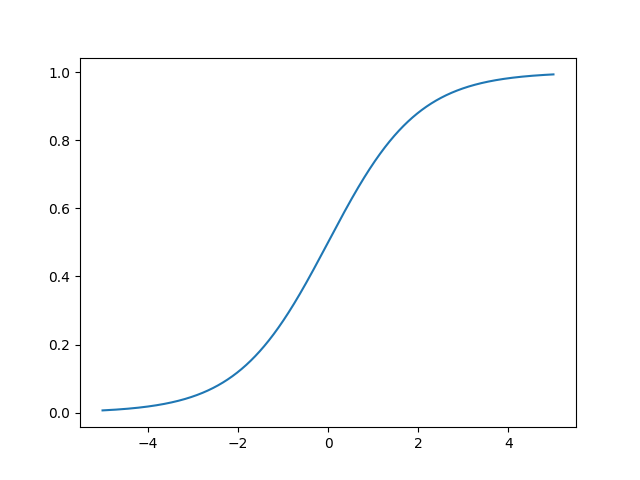
\includegraphics[scale=.4]{Images/Output/sigmoid.png}
\end{figure}
		\begin{equation}
			\sigma(x) = \frac{1}{1+e^{w_{i}^{T}x+b}}
		\end{equation}
\end{frame}


\begin{frame}[fragile]
\frametitle{Activation Functions: Tanh}
\begin{figure}
		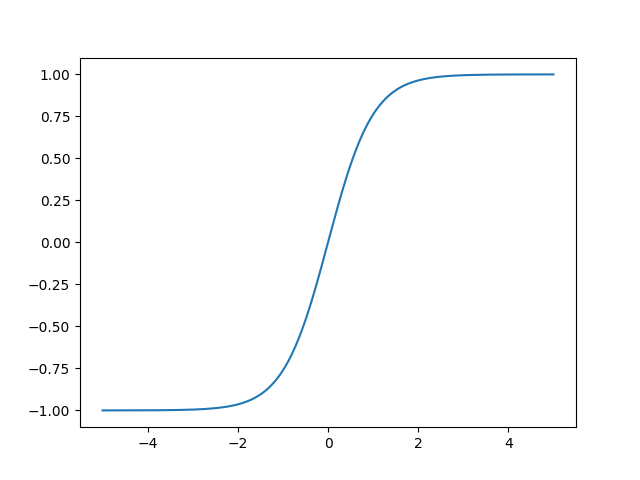
\includegraphics[scale=.4]{Images/Output/tanh.png}
\end{figure}
		\begin{equation}
			tanh(x)_i = \frac{e^{x_i}-e^{-x_i}}{e^{x_i}+e^{+x_i}}
		\end{equation}
\end{frame}

\begin{frame}[fragile]
\frametitle{Activation Functions: ReLU}
\begin{figure}
		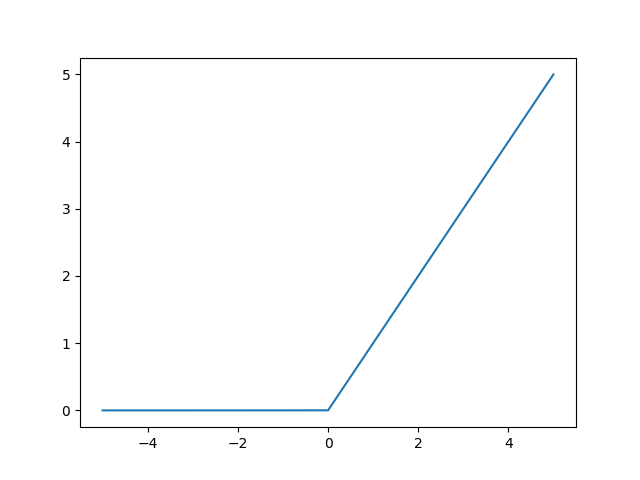
\includegraphics[scale=.4]{Images/Output/relu.png}
\end{figure}
		\begin{equation}
			f(x) = max(0,Wx+b)
		\end{equation}
\end{frame}

\begin{frame}[fragile]
\frametitle{Activation Functions: Softmax}
		\begin{equation}
			\sigma(x)_i = \frac{e^{x_i}}{\sum_{j=1}^{n}e^{x_j}}
		\end{equation}
\end{frame}


\begin{frame}[fragile]
\frametitle{Full Network}
	\begin{neuralnetwork}[height=4, layerspacing=23mm]
		\newcommand{\x}[2]{$x_#2$}
		\newcommand{\y}[2]{$\hat{y}_#2$}
		\newcommand{\hfirst}[2]{\small $h^{(1)}_#2$}
		\newcommand{\hi}[2]{\small $h^{(i)}_#2$}
		\newcommand{\hsecond}[2]{\scriptsize $h^{(n-1)}_#2$}
		\inputlayer[count=3, bias=true, title=Input\\layer, text=\x]
		\hiddenlayer[count=4, bias=true, title=\\, text=\hfirst] \linklayers
		\hiddenlayer[count=3, bias=true, title=\\i, text=\hi] \linklayers
		\hiddenlayer[count=3, bias=true, title=\\n-1, text=\hsecond] \linklayers
		\outputlayer[count=2, title=Output\\layer, text=\y] \linklayers
	    \end{neuralnetwork}
	\begin{center}
	    Prior to the activation function of nodes. Each layer undergoes a transformation into a |l+1| dimensional space.
	\end{center}
    %Now this cascade of transformations should be optimized to the training data.
\end{frame}


\begin{frame}[fragile]
	\frametitle{Training}
	\begin{figure}
		\begin{small}
			\begin{equation}
			J(W,b;x,y) = [\frac{1}{m}*\sum_{i=1}^{m} J(W,b,x^i,y^i)] + \frac{\lambda}{2}*\sum_{l=1}^{n_l-1}*\sum_{l=1}^{s_l}*\sum_{l=1}^{s_{l+1}}(W_{ji}^{(i)})^2
			\end{equation}
		\end{small}
		\caption{Cost function over a batch of m training examples ($x_i$,$y_i$) \cite{ng2011sparse}}
	\end{figure}
	No analytic solution -> Iteratively update weights
	\begin{itemize}
		\item Gradient descent w.r.t weights and bias (batch/stochastic)
		\item Newton's Method (requires Hessian) 
		\item Momentum learning ... lots of tweaks
	\end{itemize}
\end{frame}


\begin{frame}[fragile]
\frametitle{Cost Function}
	\begin{tiny}
		\begin{equation}
			J(W,b;x,y) = [\frac{1}{m}*\sum_{i=1}^{m} J(W,b,x^i,y^i)] + \frac{\lambda}{2}*\sum_{l=1}^{n_l-1}*\sum_{l=1}^{s_l}*\sum_{l=1}^{s_{l+1}}(W_{ji}^{(i)})^2
			\end{equation}
	\end{tiny}
	\normalsize
	\begin{itemize}
			%TODO: fix these up
	\item 		
		Quadratic
		\begin{equation}
			\frac{1}{m}\sum_{i=1}^{m}\frac{1}{2}||y_i - a^l_i||^{2}
		\end{equation}
	\item 
		ML parametarized model (minimum KL Divergence)  \cite{ng2011sparse}
		\begin{equation}
			(W,b)_{ML} = argmax_{W,b}Pr(Y|X,W,b)
		\end{equation}
	\end{itemize}
	\begin{small}
		Without regularization this searches for the ML model for the \textbf{training} data 
		\cite{goodfellow2016deep}
	\end{small}
\end{frame}


\begin{frame}
	\frametitle{Regularization (Training Data is Expensive)}
	ML converges asymptotically but we usually don't have infinite data so we enforce priors
\end{frame}


\subsubsection{Autoencoders}

\frame{\tableofcontents[currentsection,hideothersubsections,currentsubsection]}

\begin{frame}[fragile]
	\frametitle{Autoencoders and Source Coding}
	\begin{figure}
		\begin{neuralnetwork}[height=4, nodespacing=10mm, layerspacing=15mm]
		\newcommand{\x}[2]{$x_#2$}
		\newcommand{\y}[2]{$\hat{y}_#2$}
		\newcommand{\hfirst}[2]{\small $h^{(1)}_#2$}
		\newcommand{\hsecond}[2]{\small $h^{(2)}_#2$}
		\newcommand{\hthird}[2]{\small $h^{(3)}_#2$}
		\newcommand{\hfourth}[2]{\small $h^{(4)}_#2$}
		\newcommand{\hfifth}[2]{\small $h^{(5)}_#2$}
		\newcommand{\hsixth}[2]{\small $h^{(6)}_#2$}
		\inputlayer[count=3, bias=false, title=Input\\, text=\x]
		\hiddenlayer[count=4, bias=true, title=\\, text=\hfirst] \linklayers
		\hiddenlayer[count=3, bias=true, title=\\, text=\hsecond] \linklayers
		\hiddenlayer[count=2, bias=true, title=Compress\\, text=\hthird] \linklayers
		\hiddenlayer[count=4, bias=true, title=\\, text=\hfourth] \linklayers
		\outputlayer[count=3, title=Output\\, text=\x] \linklayers
	    \end{neuralnetwork}
	\end{figure}
	%We can take the output of an intermediate layer after training as use it as the input features for a
	%classification neural network.
\end{frame}


%Could insert a slide showing how a sparse solution could be guided via regularization

\begin{frame}[fragile]
	\frametitle{Priciple Component Analysis as an Autoencoder}
	\begin{figure}[h!]
		\begin{neuralnetwork}[height=3, nodespacing=10mm, layerspacing=35mm]
		\newcommand{\x}[2]{$x_#2$}
		\newcommand{\y}[2]{$\hat{y}_#2$}
		\newcommand{\hfirst}[2]{\small $h^{(1)}_#2$}
		\inputlayer[count=4, bias=True, title=\\, text=\x]
		\hiddenlayer[count=2, bias=false, title=Representation\\, text=\hfirst] \linklayers
		\outputlayer[count=4, title=\\, text=\x] \linklayers
	    \end{neuralnetwork}
	\end{figure}

	\begin{scriptsize}
	Of interest here is the Matrix $ W^{1} $ with elements $W_{ij}^{1}$. If we use the cost function $||h_{W,b}(x) -y||^2$, this matrix will
	span the eigenspace of the dataset similarly to the way PCA selects the span of eigenvectors corresponding to
	the largest eigenvalues.
	\end{scriptsize}
\end{frame}


\begin{frame}
	\frametitle{Interpretting Regularizing with Autoencoders}
	\begin{block}{Classification}
	%Main point of this slide is to say that in classification types of things, we can interpret regularization
	%directly as bayesian priors. 
	Regularization corresponds to priors on parameters of the training data pdf model.
	\end{block}

	\begin{block}{Autoencoder}
		%Here when we add a sparsity penalty it enforcing a prior on the latent variables of
			%the data. Note Autoencoders learn latent variables. TODO Add example regularization from Ng paper
		Autoencoders learn latent variables so regularization corresponds priors on these latent variables.
	\end{block}
\end{frame}


\begin{frame}[fragile, label=DNA]
	\frametitle{Denoising Autoencoder}
	\begin{figure}
		\begin{neuralnetwork}[height=4, nodespacing=10mm, layerspacing=20mm]
		\newcommand{\x}[2]{$x_#2$}
		\newcommand{\y}[2]{$\hat{x}_#2$}
		\newcommand{\hfirst}[2]{\small $h^{(1)}_#2$}
		\newcommand{\hsecond}[2]{\small $h^{(2)}_#2$}
		\newcommand{\hthird}[2]{\small $h^{(3)}_#2$}
		\inputlayer[count=3, bias=false, title=Input\\, text=\x]
		\hiddenlayer[count=4, bias=true, title=Encode\\, text=\hfirst] \linklayers
		\hiddenlayer[count=4, bias=true, title=Channel\\, text=\hsecond] \linklayers
		\hiddenlayer[count=4, bias=true, title=Decode\\, text=\hthird] \linklayers
		\outputlayer[count=3, title=Output\\, text=\x] \linklayers
	    \end{neuralnetwork}
	\end{figure}
%	Detail what can happen in channel -> noise and multipath delay (means we can't train training examples independently. This is
%	important as in some cases (Molecular Communications) the channel is not independent of the transmitted message CITE.
%	Encoding stage up to the part where distortion takes place, then decoding the distortion
	Channel model can impact how we train \cite{felix2018ofdm}
\end{frame}


\begin{frame}
	\frametitle{Training Deep Autoencoders}
	Individual layers are often "pre-trained" to learn an
	idea of the latent variables they should be moving towards.
%	Note that to even begin this single layer training, we need random initialization
%	in order to prevent symmetry in the activation functions and thus gradient steps of nodes in a layer
	\cite[14.3][]{goodfellow2016deep}
\end{frame}

\subsection{OFDM}

%------------------------------------------------
\subsubsection{Motivation}

\frame{\tableofcontents[currentsection,hideothersubsections,currentsubsection]}


\begin{frame}
	\frametitle{Dividing Channel Resources}
	\begin{figure}
	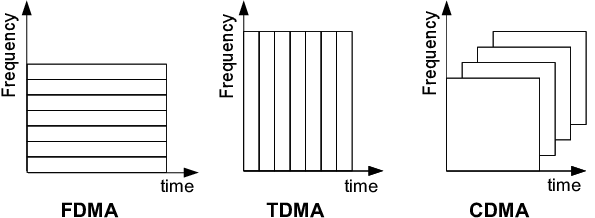
\includegraphics[scale=1]{Images/Output/FDMA-TDMA-CDMA-Frequency-Time-division.png}
		\caption{Multiple Access Schemes (include SDMA/NOMA?)}
	\end{figure}
\end{frame}


\begin{frame}[squeeze]
\frametitle{Sinusoids in LTI systems}

	\begin{figure}
			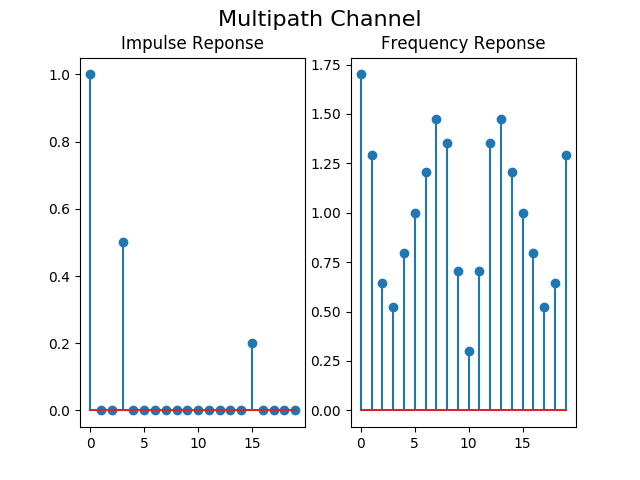
\includegraphics[scale=.4, height=2cm]{Images/Output/Multipath_Channel.png}
		\caption{Multipath Channel}
	\end{figure}

%		\begin{block}{Takeaway}
%			Perfect sinusoids through a multipath channel, can be easily equalized with a single multiplication
%			so we can modulate with qam and be
%			sure to reverse the effects of the channel to find the
%			transmitted information
%		\end{block}
%
%		\begin{block}{Problem}
%			An infinite sinusoid does not convey information
%		\end{block}

			\begin{equation*}
				x(t) = e^{j2\pi f_c t}
			\end{equation*}

			\begin{equation*}
				\sum_{n=1}^{n} c_n*\delta(t-\tau_n)
			\end{equation*}
\end{frame}

\begin{frame}
	\begin{block}{Solution step 1}
		Truncate the sinusoid with a rectangular window in time...
		Convolves frequency with sinc
	\end{block}

	\begin{block}{Solution step 2}
		In discrete time, a finite sinusoid can still be represented by a
		delta in discrete frequency.
	\end{block}

\end{frame}

\begin{frame}[label=OFDM]
	\frametitle{OFDM Outline}
	\begin{figure}
		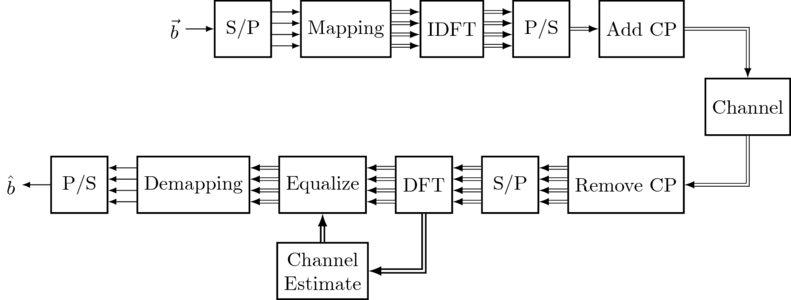
\includegraphics[scale=.4]{Images/Output/ofdm.png}
		\caption{\footcite{ofdmillustration}}
	\end{figure}
	Discrete frequency  multiplied by channel frequency response -> circular convolution in time.
\end{frame}

\begin{frame}
	\frametitle{Multiplexing}
	\begin{block}{ORTHOGONAL Frequency Division MULTIPLEXING}
		N-point time sample contains N frequencies at modulated phase/magnitude. 
		The result can carry information on all N \underline{orthogonal} sinusoids.
	\end{block}
	*Users are assigned to sets of frequencies within an N-point DFT.
\end{frame}

\begin{frame}
	\frametitle{Synchonization }
	%\begin{equation}
	Orthogonality of the N "sub-carriers" depends on equally spaced samples.
	%\end{equation}

	Sampling period and total number of samples need to be synchronized to preserve sub-carrier orthogonality. 
	This results in strict requirements on transmit/receive oscillator synchronization.
	-Show how synchronization mismatch can cause problems
	Just include this with mention that it will be important for next section
	\cite{sandell1995timing}
\end{frame}



\subsubsection{Pros and Cons to OFDM}

\begin{frame}
	\frametitle{Benefits and drawbacks}
	\begin{itemize}
		\item Large Peak to Average Power Ratio (\textbf{PAPR})
			\begin{itemize}
				\item{Variance of single die roll: PAPR = 2.37
					\begin{equation}
						E[|x|^2] = 15.166
					\end{equation}}

				\item{Variance of sum of two dice rolled: PAPR = 2.62
					\begin{equation}
						E[|x_1+x_2|^2] = 54.833
					\end{equation}}
			\end{itemize}
		
		\item Cycle Prefix overheard proportional to channel response length

		\item Sensitive to asynchronous transmission

	\end{itemize}
\end{frame}

\begin{frame}
\frametitle{Current Deployment of OFDM}
	
\end{frame}


%------------------------------------------------
\section{Putting it together}
%------------------------------------------------

\subsection{OFDM + Autoendcoder}


\frame{\tableofcontents[currentsection,hideothersubsections]}

%Point of this slide is to recall what a full autoencoder implementation of the communication system would look like
%\againframe{DNA}

\begin{frame}[label=OFDM]
	\frametitle{OFDM Outline}
	\begin{figure}
		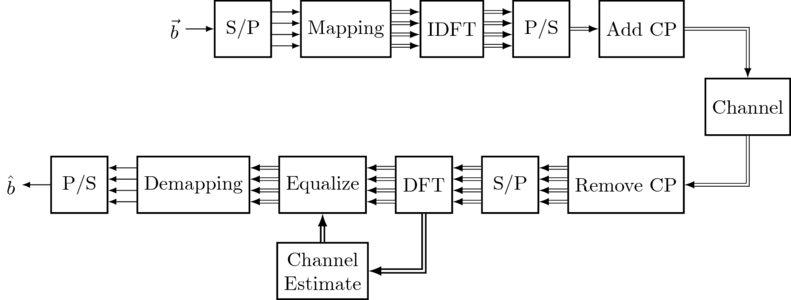
\includegraphics[scale=.4]{Images/Output/ofdm.png}
	\end{figure}
\end{frame}


\begin{frame}[label=OFDM]
	\frametitle{End-to-End Autoencoder}
	\begin{figure}[t]
		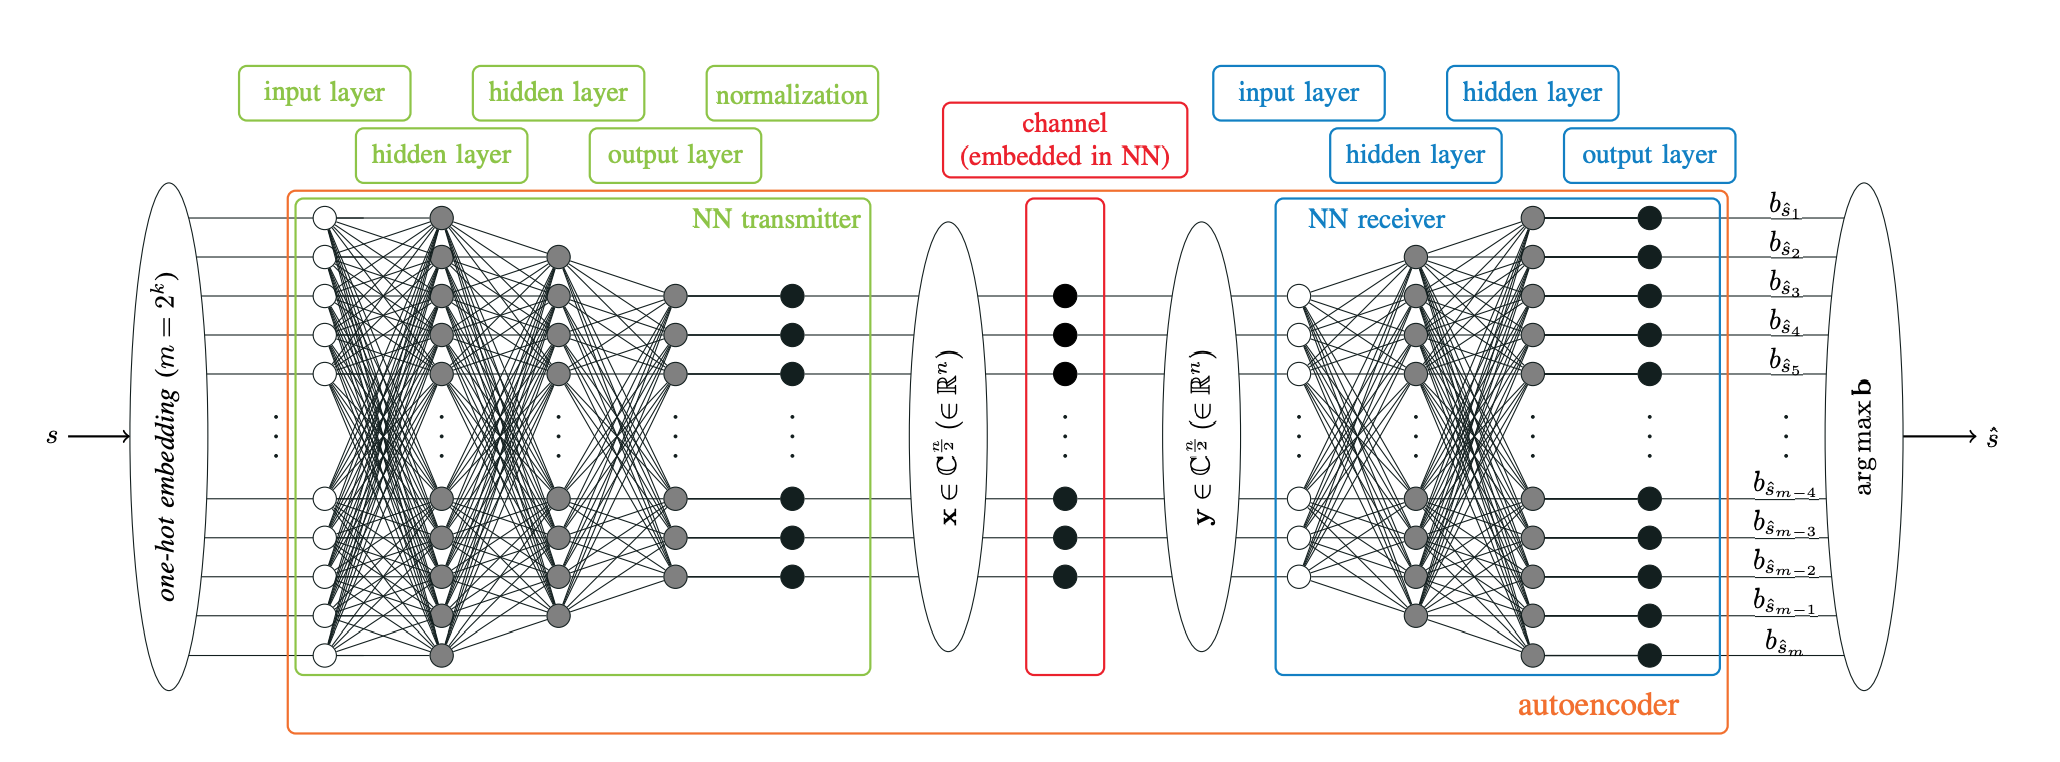
\includegraphics[scale=.4]{Images/endtoend.png}
		\centering
		\caption{\footcite{felix2018ofdm}}
	\end{figure}
	\begin{itemize}
		\item normalization layer
		\item sequence detector  -> based on channel length (why would this be needed in OFDM?)
		\item discuss difficulties implied by continuous transmission a
	\end{itemize}
\end{frame}



\subsubsection{Previous Work}

\begin{frame}
	\frametitle{Naive Modeling}
	Intuitively this gives the network freedom to learn the best channel equalization. Classifying will require the
	network to perform a marginalization over all variables in the channel.
	%Observed to be difficult in intial work
\end{frame}

\begin{frame}
	\frametitle{Synchonization}
	Why this might be difficult. Resolved in previous work using additional NN.
	OFDM allows for simple sampling synchronization using autocorrelation with the cyclic prefix.
\end{frame}



\subsubsection{Setup for integrating OFDM into the NN}

\begin{frame}
	\frametitle{Applying domain knowledge to NN Architectures}
	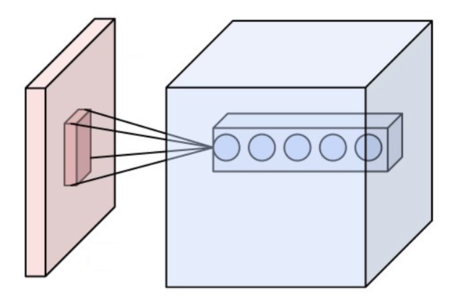
\includegraphics[scale=.25]{Images/Conv_layer.png}
	\begin{itemize}
		\item Reduce required training data and increase training speed
		\item Improved generalization
	\end{itemize}
\end{frame}

\begin{frame}
	\frametitle{RTN -- OFDM}
	We take length $w_{fft}$ inverse fft over $w_{fft}$ messages with each message being length $\frac{n}{2}$ long. The
	result is that we send $\frac{n}{2}$ symbols over each carrier in the multicarrier system. All $\frac{n}{2}$ can be
	equalized with the same pilot.
\end{frame}

\begin{frame}
	\frametitle{Channel Model}
	
\end{frame}


\begin{frame}
	\frametitle{Training}
	Discuss the two stages of training
\end{frame}

\begin{frame}
	\frametitle{Sequence Detector}
\end{frame}

\begin{frame}
	\frametitle{Equalization}
	\begin{itemize}
		\item Pilot tones with MMSE Equalizer
		\item Pilot tones without explicit equalizer
		\item No pilot or explicit equalizer
	\end{itemize}
\end{frame}

\subsection{ViterbiNet}


\frame{\tableofcontents[currentsection,hideothersubsections,currentsubsection]}

\begin{frame}
Normally we have models for the channels and these models usually incorporate random variables as parameters.The current state of the channel is one realization of these random parameters

Pure ML approach no longer assumes a specific model until trained

This study considers the case in which we assume a model but allow for estimation of model parameters

Each decoded block provides information with which to update the model



	End result achieves similar performance to CSI based (~?? dB)
	ViterbiNet outperforms standard Viterbi when there is CSI uncertainty (uncoded)
\begin{equation}
	\hat{s}(y) = argmin_s\sum_{i=1}^{t}-log(P_{Y[i]|s}(y[i]|s)
\end{equation}
	Knowing $-log(P_{Y[i]|s}(y[i]|s)$ provides metrics for Viterbi trellis
	Discuss the two stages of training

	Further work for online training utilizing FEC to provide a new source of training data
\end{frame}

\section{Conclusion}

\begin{frame}
\frametitle{Future Directions}
\begin{large}

\end{large}
\end{frame}

\begin{frame}
\frametitle{Question?}
\begin{large}

\end{large}
\end{frame}

\begin{frame}
\begin{tiny}
	\printbibliography[title={Whole bibliography}]

\end{tiny}
\end{frame}

\end{document} 